% !TEX root = ../notes_unsupervisedlearning.tex
% Chapter 7: Anomaly Detection and Evaluation
%%%%%%%%%%%%%%%%%%%%%%%%%%%%%%%%%%%%%%%%%%%%%%%%%%%%%%%%%%%%%%%%%%%%%%

\chapter{Anomaly Detection and Evaluation}\index{Anomaly Detection}\index{OOD Detection}
\newthought{Structure reveals itself through deviations.}

%═══════════════════════════════════════════════════════════════════════
% BLOCK 1: INTRODUCTION
%═══════════════════════════════════════════════════════════════════════

\section{The Why}

\marginnote{The unusual is often the important: fraud, disease, defects, discoveries.}

Once we've modeled "normal" data, we can detect what \textbf{doesn't fit}. Anomaly detection is critical for:
\begin{itemize}
    \item \textbf{Fraud detection}: Unusual transactions in banking
    \item \textbf{Medical diagnosis}: Abnormal scans or lab results
    \item \textbf{Manufacturing}: Defective products on assembly lines
    \item \textbf{Cybersecurity}: Intrusion detection, malware identification
    \item \textbf{Scientific discovery}: Finding rare events in particle physics
\end{itemize}

\textbf{The challenge}: Anomalies are rare (often $<1\%$) and undefined---we can't enumerate all possible anomalies.

\subsection{Hands-On Experience}

\begin{marginfigure}
\begin{tikzpicture}[scale=0.7]
    \begin{axis}[
        xlabel={$x_1$},
        ylabel={$x_2$},
        xmin=-1, xmax=8,
        ymin=-1, ymax=6,
        width=\textwidth,
        height=\textwidth,
    ]
    % Normal cluster
    \addplot[only marks, mark=*, mark size=2pt, blue] coordinates {
        (2,2) (2.5,2.3) (2.2,2.8) (3,2.5) (2.8,2) (2.3,2.5)
        (2.7,2.2) (2.4,2.7) (2.1,2.4) (2.6,2.6)
    };
    % Anomalies
    \addplot[only marks, mark=*, mark size=3pt, red] coordinates {
        (6,1) (1,5) (7,4)
    };
    % Labels
    \node[blue] at (axis cs:2.5,1) {Normal};
    \node[red] at (axis cs:6,0.3) {?};
    \node[red] at (axis cs:1,5.5) {?};
    \node[red] at (axis cs:7,4.5) {?};
    \end{axis}
\end{tikzpicture}
\caption{Which points are anomalies? On what basis?}
\end{marginfigure}

Given a cluster of "normal" points, consider:
\begin{enumerate}
    \item Point at $(6, 1)$: Far from cluster. Anomaly score?
    \item Point at $(2.5, 2.5)$: Center of cluster. Anomaly score?
    \item What threshold would you use to classify as anomaly?
\end{enumerate}

\subsection{Learning Objectives}

After this lecture, you will be able to:
\begin{enumerate}
    \item Distinguish point, contextual, and collective anomalies
    \item Apply statistical, proximity-based, and reconstruction-based methods
    \item Implement uncertainty estimation using Monte Carlo Dropout
    \item Evaluate clustering quality without ground truth labels
    \item Design graceful degradation strategies for deployed models
\end{enumerate}

%═══════════════════════════════════════════════════════════════════════
% BLOCK 2: MAIN THEORY
%═══════════════════════════════════════════════════════════════════════

\section{Types of Anomalies}

\marginnote{Not all anomalies are created equal.}

\begin{description}
    \item[Point anomalies] Individual instances that are anomalous with respect to the rest. \textit{Example: A single fraudulent transaction.}

    \item[Contextual anomalies] Instances anomalous in a specific context but not otherwise. \textit{Example: 30°C is normal in summer, anomalous in winter.}

    \item[Collective anomalies] A collection of instances that together are anomalous. \textit{Example: A sequence of normal login attempts from 100 different countries in 1 hour.}
\end{description}

\begin{figure}[h]
\centering
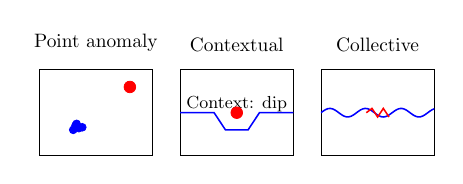
\begin{tikzpicture}[scale=0.7]
    % Point anomaly
    \begin{axis}[
        name=point,
        title={Point anomaly},
        xmin=0, xmax=10, ymin=0, ymax=10,
        width=0.3\textwidth,
        ticks=none,
    ]
    \addplot[only marks, mark=*, mark size=2pt, blue] coordinates {
        (3,3) (3.5,3.2) (3.2,3.5) (3.8,3.3) (3.3,3.7)
    };
    \addplot[only marks, mark=*, mark size=3pt, red] coordinates {(8,8)};
    \end{axis}

    % Contextual anomaly
    \begin{axis}[
        at={(point.east)}, anchor=west, xshift=0.5cm,
        name=context,
        title={Contextual},
        xmin=0, xmax=10, ymin=0, ymax=10,
        width=0.3\textwidth,
        ticks=none,
    ]
    \addplot[blue, thick] coordinates {(0,5) (3,5) (4,3) (6,3) (7,5) (10,5)};
    \addplot[only marks, mark=*, mark size=3pt, red] coordinates {(5,5)};
    \node at (axis cs:5,6) {\small Context: dip};
    \end{axis}

    % Collective anomaly
    \begin{axis}[
        at={(context.east)}, anchor=west, xshift=0.5cm,
        title={Collective},
        xmin=0, xmax=10, ymin=0, ymax=10,
        width=0.3\textwidth,
        ticks=none,
    ]
    \addplot[blue, thick, domain=0:10, samples=50] {5 + 0.5*sin(deg(x*2))};
    \addplot[red, thick] coordinates {(4,5) (4.5,5.5) (5,4.5) (5.5,5.5) (6,4.5)};
    \end{axis}
\end{tikzpicture}
\caption{Three types of anomalies: point (isolated), contextual (wrong context), collective (unusual pattern).}
\end{figure}


\section{Statistical Methods}

\marginnote{Parametric: assume a distribution, flag low-probability points.}

\subsection{Z-Score}

For univariate data:
\begin{equation}
    z_i = \frac{x_i - \mu}{\sigma}
\end{equation}

Flag as anomaly if $|z_i| > 3$ (or other threshold). Assumes normality.

\subsection{Gaussian Mixture Model Likelihood}

Fit a GMM, compute likelihood:
\begin{equation}
    p(x) = \sum_{k=1}^K \pi_k \mathcal{N}(x | \mu_k, \Sigma_k)
\end{equation}

Low $p(x)$ indicates anomaly.

\subsection{Extreme Value Theory}

For heavy-tailed distributions, model the tail explicitly using Generalized Pareto Distribution:
\begin{equation}
    F(x) = 1 - \left(1 + \frac{\xi x}{\sigma}\right)^{-1/\xi}
\end{equation}


\section{Proximity-Based Methods}

\subsection{k-NN Distance}

\marginnote{Simple and effective: anomalies are far from their neighbors.}

Anomaly score = distance to $k$-th nearest neighbor.

\begin{equation}
    \text{score}(x) = d(x, x^{(k)})
\end{equation}

where $x^{(k)}$ is the $k$-th nearest neighbor of $x$.

\subsection{Local Outlier Factor (LOF)}

\marginnote{LOF compares local density to neighbors' density.}

LOF accounts for varying density:
\begin{equation}
    \text{LOF}_k(x) = \frac{\sum_{y \in N_k(x)} \text{lrd}_k(y) / \text{lrd}_k(x)}{|N_k(x)|}
\end{equation}

where $\text{lrd}_k(x)$ is the local reachability density. LOF $\approx 1$ means similar density to neighbors; LOF $\gg 1$ means lower density (anomaly).

\begin{figure}[h]
\centering
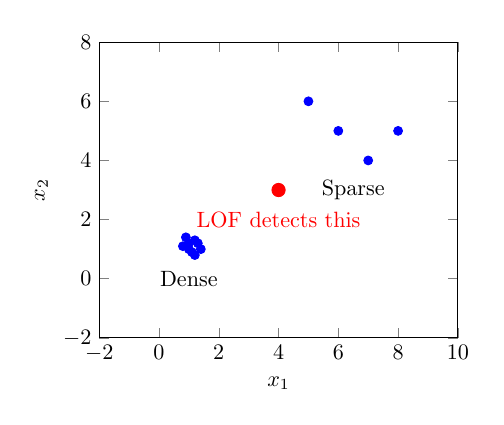
\begin{tikzpicture}[scale=0.8]
    \begin{axis}[
        xlabel={$x_1$}, ylabel={$x_2$},
        xmin=-2, xmax=10, ymin=-2, ymax=8,
        width=0.6\textwidth,
    ]
    % Dense cluster
    \addplot[only marks, mark=*, mark size=2pt, blue] coordinates {
        (1,1) (1.2,1.3) (0.8,1.1) (1.1,0.9) (1.3,1.2)
        (0.9,1.4) (1.4,1.0) (1.0,1.2) (1.2,0.8)
    };
    % Sparse cluster
    \addplot[only marks, mark=*, mark size=2pt, blue] coordinates {
        (6,5) (7,4) (5,6) (8,5)
    };
    % Anomaly in sparse region
    \addplot[only marks, mark=*, mark size=3pt, red] coordinates {(4,3)};
    % Labels
    \node at (axis cs:1,0) {Dense};
    \node at (axis cs:6.5,3) {Sparse};
    \node[red] at (axis cs:4,2) {LOF detects this};
    \end{axis}
\end{tikzpicture}
\caption{LOF detects the anomaly despite varying cluster densities.}
\end{figure}


\section{Reconstruction-Based Methods}

\marginnote{If the model can't reconstruct it, it's probably anomalous.}

\subsection{Autoencoder Reconstruction Error}

Train autoencoder on normal data. Anomaly score:
\begin{equation}
    \text{score}(x) = \|x - \text{decode}(\text{encode}(x))\|^2
\end{equation}

High reconstruction error indicates the model hasn't learned to represent this type of data.

\subsection{VAE Log-Likelihood}

Use the ELBO as anomaly score:
\begin{equation}
    \text{score}(x) = -\text{ELBO}(x) = -\mathbb{E}_{q(z|x)}[\log p(x|z)] + D_{KL}(q(z|x) \| p(z))
\end{equation}


\section{Uncertainty Estimation}

\marginnote{Knowing what you don't know is crucial for safe AI.}

\subsection{Types of Uncertainty}

\begin{description}
    \item[Aleatoric] Inherent noise in data (irreducible)
    \item[Epistemic] Model uncertainty due to limited data (reducible with more data)
\end{description}

\subsection{Monte Carlo Dropout}

\begin{algorithm}[H]
\caption{MC Dropout for Uncertainty}
\begin{algorithmic}[1]
\Require Input $x$, model with dropout, $T$ forward passes
\For{$t = 1$ to $T$}
    \State $\hat{y}_t \gets$ forward pass with dropout enabled
\EndFor
\State Mean prediction: $\bar{y} = \frac{1}{T} \sum_t \hat{y}_t$
\State Uncertainty: $\text{Var}(\hat{y}) = \frac{1}{T} \sum_t (\hat{y}_t - \bar{y})^2$
\end{algorithmic}
\end{algorithm}

High variance indicates high epistemic uncertainty---the model is unsure.

\subsection{Deep Ensembles}

Train $M$ models independently, aggregate predictions:
\begin{equation}
    p(y|x) = \frac{1}{M} \sum_{m=1}^M p_m(y|x)
\end{equation}

Disagreement among ensemble members indicates uncertainty.


\section{Out-of-Distribution Detection}

\marginnote{OOD detection: is this input from the training distribution?}

\subsection{Softmax Confidence (and its failures)}

Naive approach: flag low-confidence predictions.
\begin{equation}
    \text{score}(x) = \max_k p(y=k|x)
\end{equation}

\textbf{Problem}: Neural networks are often confidently wrong on OOD data!

\subsection{ODIN}

Temperature scaling + input perturbation:
\begin{equation}
    \tilde{x} = x - \epsilon \cdot \text{sign}(\nabla_x \log p(y=\hat{y}|x; T))
\end{equation}

\subsection{Energy-Based OOD Detection}

Use the energy function:
\begin{equation}
    E(x) = -\log \sum_k \exp(f_k(x))
\end{equation}

Higher energy indicates OOD.


\section{Evaluation Without Labels}

\marginnote{How do we evaluate unsupervised methods without ground truth?}

For clustering evaluation:

\subsection{Silhouette Score}

\begin{equation}
    s(i) = \frac{b(i) - a(i)}{\max(a(i), b(i))}
\end{equation}

Average over all points. Range: $[-1, 1]$, higher is better.

\subsection{Calinski-Harabasz Index}

Ratio of between-cluster to within-cluster dispersion:
\begin{equation}
    CH = \frac{SS_B / (K-1)}{SS_W / (N-K)}
\end{equation}

Higher is better.

\subsection{Stability Analysis}

\begin{enumerate}
    \item Run clustering multiple times (different initializations, subsamples)
    \item Measure consistency of assignments
    \item Stable clusters are more reliable
\end{enumerate}


\section{Graceful Degradation}

\marginnote{Safe AI: know when to hand off to humans.}

When deploying ML systems:

\begin{enumerate}
    \item \textbf{Confidence thresholds}: Only act on high-confidence predictions
    \item \textbf{Human handoff}: Route uncertain cases to human reviewers
    \item \textbf{Fail-safe defaults}: When uncertain, take the safe action
    \item \textbf{Monitoring}: Track prediction confidence over time; alert on distribution shift
\end{enumerate}


%═══════════════════════════════════════════════════════════════════════
% BLOCK 3: STUDENT ACTIVATION
%═══════════════════════════════════════════════════════════════════════

\section{Examples \& Exercises}

\subsection{Exercise 1: LOF Computation}

Given 5 points: $A=(0,0)$, $B=(1,0)$, $C=(0,1)$, $D=(1,1)$, $E=(5,5)$

With $k=2$:
\begin{enumerate}
    \item Compute the 2-distance for each point
    \item Which point has the highest LOF?
\end{enumerate}

\textbf{Solution}: Points A-D form a tight cluster (distances $\approx 1$). Point E is far from all others (distance to nearest $\approx 5.7$). E will have LOF $\gg 1$.

\subsection{Exercise 2: Reconstruction Anomaly}

You train an autoencoder on MNIST digits 0-8. At test time, you see digit 9.

\begin{enumerate}
    \item What reconstruction error do you expect?
    \item Why might the autoencoder still produce a low error?
\end{enumerate}

\textbf{Solution}:
\begin{enumerate}
    \item High error---the model never learned to encode/decode 9.
    \item The autoencoder might reconstruct 9 as a similar-looking digit (4 or 7), producing moderate error. This is a failure mode.
\end{enumerate}

\subsection{Exercise 3: Silhouette Score}

A clustering has 3 points in cluster A: $(0,0), (1,0), (0,1)$ and 2 points in cluster B: $(5,5), (6,5)$.

Compute the silhouette score for point $(0,0)$.

\textbf{Solution}:
\begin{itemize}
    \item $a(0,0)$ = mean distance within cluster = $(1 + 1)/2 = 1$
    \item $b(0,0)$ = mean distance to cluster B = $(\sqrt{50} + \sqrt{61})/2 \approx 7.44$
    \item $s = (7.44 - 1) / 7.44 \approx 0.87$ (well-clustered)
\end{itemize}


\section{Self-Reflection \& Recap}

\subsection{Reflection Questions}
\begin{enumerate}
    \item Why might high softmax confidence not indicate in-distribution data?
    \begin{quote}
        \textit{Neural networks extrapolate wildly outside training distribution, often producing confident but wrong predictions. The softmax normalizes to sum to 1 regardless of how far from training data.}
    \end{quote}

    \item How do you set an anomaly threshold in practice?
    \begin{quote}
        \textit{Use domain knowledge, validation set with known anomalies, or target a specific false positive rate. Often iteratively refined based on operational feedback.}
    \end{quote}
\end{enumerate}

\subsection{Key Concepts}
\begin{itemize}
    \item Anomalies are defined relative to a notion of "normal"
    \item Different methods capture different anomaly types
    \item \textbf{Uncertainty quantification} is crucial for safe deployment
    \item \textbf{Internal evaluation metrics} are imperfect but useful
    \item \textbf{Graceful degradation} handles cases the model can't
\end{itemize}

\subsection{Next Chapter Teaser}
\marginnote{Teaser: From detecting deviations to learning representations}
\newthought{We've seen how models can detect what they don't know.} But how do we learn good representations in the first place---without any labels at all? The next chapter explores \textbf{self-supervised learning}: using the data itself to create supervision.
